\documentclass[border=12pt]{standalone}
\usepackage{tikz}
\usetikzlibrary{positioning, calc, fit, backgrounds}
\usepackage{amsmath, amssymb}

%% ---- Hand-drawn arrowheads (filled triangles, no TikZ arrow tips) ----
%%   ahw = half-width, ahh = full height
\def\ahw{0.10}   % 1.8 mm half-width  →  3.6 mm total base
\def\ahh{0.30}   % 4.0 mm height
\def\ahws{0.1}  % smaller variant for residual arrows
\def\ahhs{0.1}

\newcommand{\arrup}[1]{% ▲ tip touching anchor, body below
  \fill[black!55] (#1) -- ++(-\ahw, -\ahh) -- ++({2*\ahw}, 0) -- cycle;}
\newcommand{\arrdown}[1]{% ▼ tip touching anchor, body above
  \fill[black!55] (#1) -- ++(-\ahw, \ahh) -- ++({2*\ahw}, 0) -- cycle;}
\newcommand{\arrleft}[1]{% ◀ tip touching anchor, body to right
  \fill[black!45] (#1) -- ++(\ahhs, \ahws) -- ++(0, {-2*\ahws}) -- cycle;}

\begin{document}
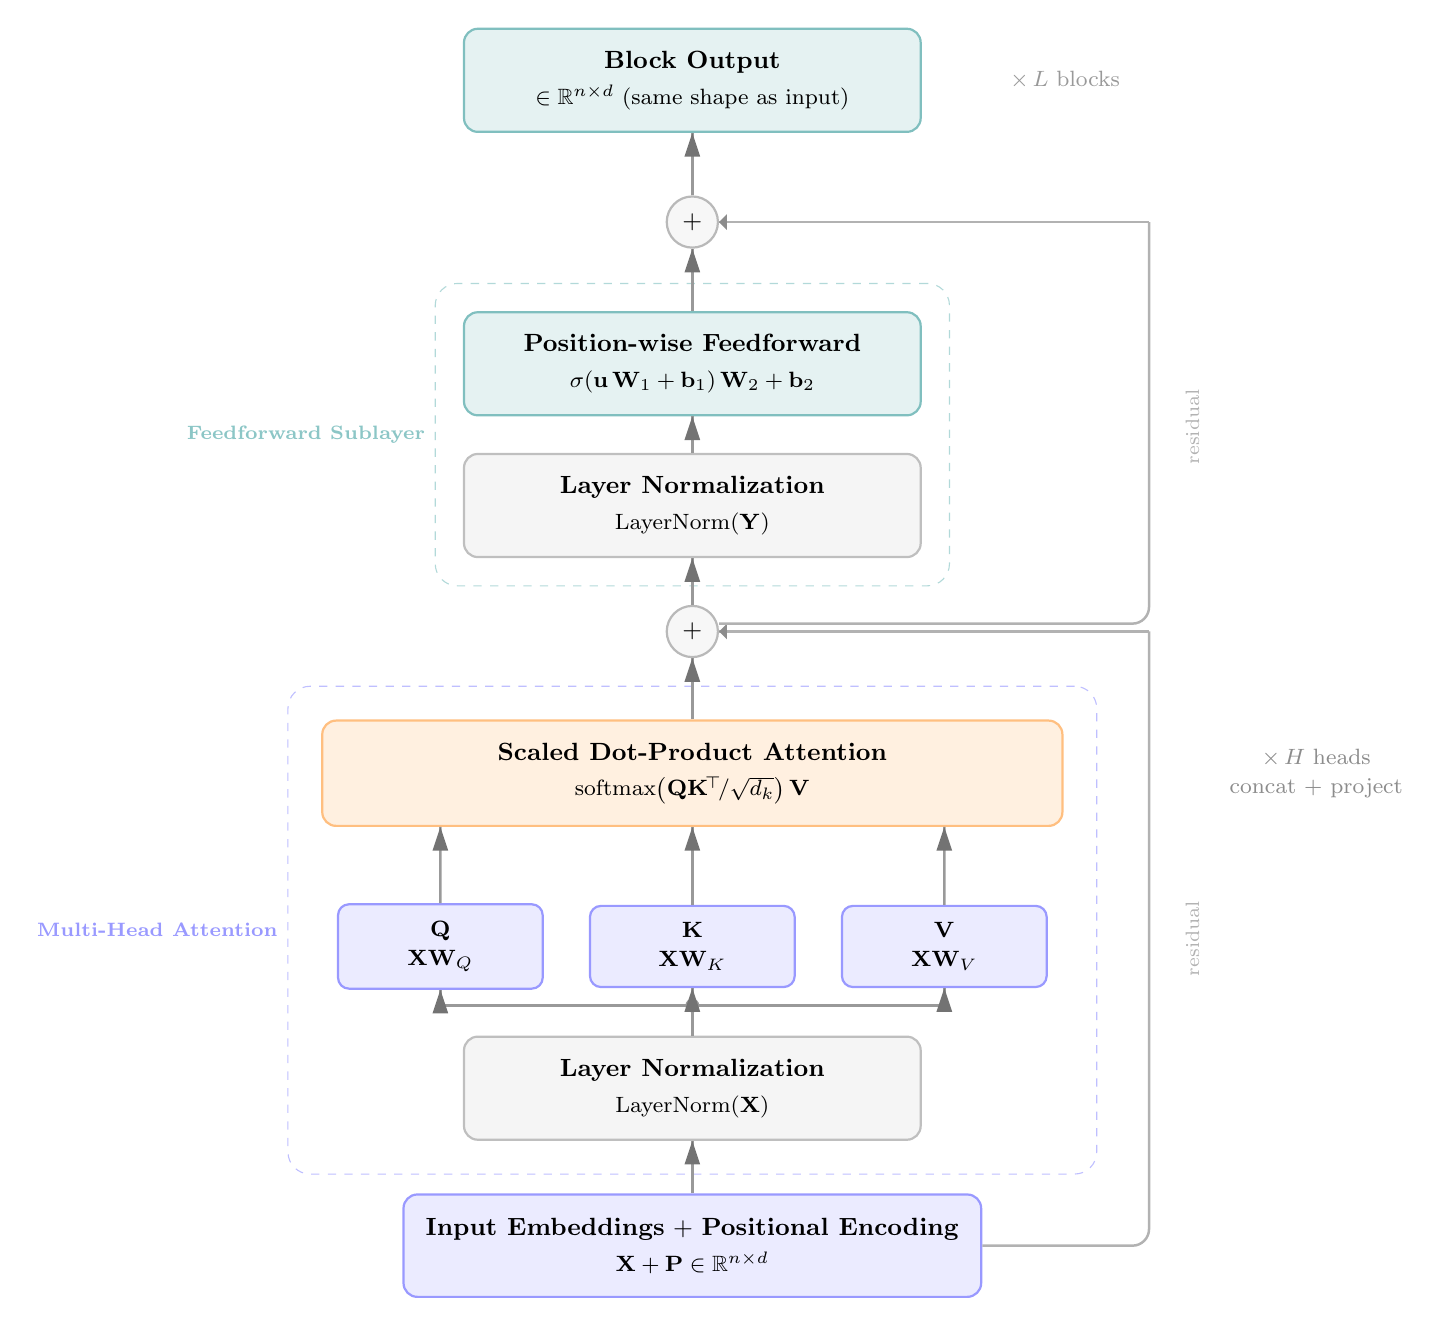
\begin{tikzpicture}[
    block/.style = {rectangle, draw=gray!60, thick, rounded corners=5pt,
                    minimum height=1.3cm, minimum width=5.8cm,
                    font=\small, inner sep=8pt, align=center},
    smallblock/.style = {rectangle, draw=gray!50, thick, rounded corners=4pt,
                    minimum height=1.0cm, minimum width=2.6cm,
                    font=\footnotesize, inner sep=6pt, align=center},
    conn/.style  = {line width=0.9pt, draw=black!40},
    resconn/.style = {line width=0.9pt, draw=black!30, rounded corners=6pt},
    plus/.style  = {circle, draw=gray!55, thick, fill=gray!6,
                    minimum size=0.65cm, font=\small, inner sep=0pt},
    lbl/.style   = {font=\footnotesize, text=black!50, align=center},
]

%% ---- Layout coordinates (Pre-Norm architecture) ----
%%   LN appears BEFORE each sublayer, residual bypasses LN+sublayer
\def\yInput{0}
\def\yLNA{2.0}       % LayerNorm before attention
\def\yQKV{3.8}
\def\yAttn{6.0}
\def\yAddA{7.8}      % first residual add
\def\yLNB{9.4}       % LayerNorm before FFN
\def\yFF{11.2}
\def\yAddB{13.0}     % second residual add
\def\yOut{14.8}
\def\resoff{5.8}

%% ==================================================================
%% NODES
%% ==================================================================

\node[block, fill=blue!8, draw=blue!40] (input) at (0, \yInput)
    {\textbf{Input Embeddings} + \textbf{Positional Encoding}\\[2pt]
     {\footnotesize $\mathbf{X} + \mathbf{P}\in\mathbb{R}^{n\times d}$}};

%% LayerNorm 1 (before attention)
\node[block, fill=gray!8, draw=gray!50, minimum width=5.8cm] (ln1)
    at (0, \yLNA)
    {\textbf{Layer Normalization}\\[2pt]
     {\footnotesize $\operatorname{LayerNorm}(\mathbf{X})$}};

%% Q, K, V projections
\node[smallblock, fill=blue!8, draw=blue!40] (wq) at (-3.2, \yQKV)
    {\textbf{Q}\\[1pt]$\mathbf{X}\mathbf{W}_{Q}$};
\node[smallblock, fill=blue!8, draw=blue!40] (wk) at (0, \yQKV)
    {\textbf{K}\\[1pt]$\mathbf{X}\mathbf{W}_{K}$};
\node[smallblock, fill=blue!8, draw=blue!40] (wv) at (3.2, \yQKV)
    {\textbf{V}\\[1pt]$\mathbf{X}\mathbf{W}_{V}$};

%% Attention
\node[block, fill=orange!12, draw=orange!50, minimum width=9.4cm] (attn)
    at (0, \yAttn)
    {\textbf{Scaled Dot-Product Attention}\\[2pt]
     {\footnotesize $\operatorname{softmax}\!\left(\mathbf{Q}\mathbf{K}^{\!\top}
      \!/\sqrt{d_{k}}\right)\mathbf{V}$}};

%% Add 1 (first residual connection)
\node[plus] (add1) at (0, \yAddA) {$+$};

%% LayerNorm 2 (before FFN)
\node[block, fill=gray!8, draw=gray!50, minimum width=5.8cm] (ln2)
    at (0, \yLNB)
    {\textbf{Layer Normalization}\\[2pt]
     {\footnotesize $\operatorname{LayerNorm}(\mathbf{Y})$}};

%% Feedforward
\node[block, fill=teal!10, draw=teal!50] (ff) at (0, \yFF)
    {\textbf{Position-wise Feedforward}\\[2pt]
     {\footnotesize $\sigma(\mathbf{u}\,\mathbf{W}_{1}
      + \mathbf{b}_{1})\,\mathbf{W}_{2} + \mathbf{b}_{2}$}};

%% Add 2 (second residual connection)
\node[plus] (add2) at (0, \yAddB) {$+$};

%% Output
\node[block, fill=teal!10, draw=teal!50] (output) at (0, \yOut)
    {\textbf{Block Output}\\[2pt]
     {\footnotesize $\in\mathbb{R}^{n\times d}$ (same shape as input)}};

%% ==================================================================
%% CONNECTIONS  (line + manual arrowhead at destination)
%% ==================================================================

%% ---- Input -> LN1 ----
\draw[conn] (input.north) -- (ln1.south);  \arrup{ln1.south}

%% ---- Fan-out: LN1 -> Q, K, V ----
\coordinate (branch) at (0, {0.5*(\yLNA + \yQKV) + 0.15});
\draw[conn] (ln1.north) -- (branch);
\fill[black!40] (branch) circle (2.5pt);
\draw[conn] (branch) -- (-3.2, {0.5*(\yLNA + \yQKV) + 0.15});
\draw[conn] (branch) -- ( 3.2, {0.5*(\yLNA + \yQKV) + 0.15});
\draw[conn] (-3.2, {0.5*(\yLNA + \yQKV) + 0.15}) -- (wq.south);   \arrup{wq.south}
\draw[conn] (0,    {0.5*(\yLNA + \yQKV) + 0.15}) -- (wk.south);   \arrup{wk.south}
\draw[conn] ( 3.2, {0.5*(\yLNA + \yQKV) + 0.15}) -- (wv.south);   \arrup{wv.south}

%% ---- Q, K, V -> Attention ----
\draw[conn] (wq.north) -- ([xshift=-3.2cm]attn.south);
\arrup{[xshift=-3.2cm]attn.south}
\draw[conn] (wk.north) -- (attn.south);
\arrup{attn.south}
\draw[conn] (wv.north) -- ([xshift=3.2cm]attn.south);
\arrup{[xshift=3.2cm]attn.south}

%% ---- Attention -> Add1 ----
\draw[conn] (attn.north) -- (add1.south);   \arrup{add1.south}

%% ---- Add1 -> LN2 -> FF -> Add2 -> Output ----
\draw[conn] (add1.north) -- (ln2.south);    \arrup{ln2.south}
\draw[conn] (ln2.north)  -- (ff.south);     \arrup{ff.south}
\draw[conn] (ff.north)   -- (add2.south);   \arrup{add2.south}
\draw[conn] (add2.north) -- (output.south); \arrup{output.south}

%% ---- Residual 1: Input bypasses LN1+Attention -> Add1 ----
\draw[resconn] (input.east) -- (\resoff, \yInput)
    -- (\resoff, \yAddA);
\draw[line width=0.9pt, draw=black!30]
    (\resoff, \yAddA) -- (add1.east);
\arrleft{add1.east}
\node[lbl, font=\scriptsize, text=black!30]
    at (\resoff + 0.55, {0.5*(\yInput + \yAddA)})
    {\rotatebox{90}{residual}};

%% ---- Residual 2: Add1 output bypasses LN2+FFN -> Add2 ----
\draw[resconn] ([yshift=0.1cm]add1.east) -- (\resoff, {\yAddA + 0.1})
    -- (\resoff, \yAddB);
\draw[line width=0.9pt, draw=black!30]
    (\resoff, \yAddB) -- (add2.east);
\arrleft{add2.east}
\node[lbl, font=\scriptsize, text=black!30]
    at (\resoff + 0.55, {0.5*(\yAddA + \yAddB)})
    {\rotatebox{90}{residual}};

%% ==================================================================
%% ANNOTATIONS
%% ==================================================================

\node[lbl, text=black!45, anchor=west] at (\resoff + 0.9, \yAttn)
    {$\times\, H$ heads\\[1pt]concat + project};

\node[lbl, text=black!40, right=1.0cm of output]
    {$\times\, L$ blocks};

%% ==================================================================
%% GROUPING BOXES
%% ==================================================================
\begin{scope}[on background layer]
    \node[draw=blue!25, dashed, rounded corners=8pt, inner sep=12pt,
          fit=(ln1)(wq)(wk)(wv)(attn),
          label={[font=\scriptsize\bfseries, blue!40]left:%
                 Multi-Head Attention}] {};
    \node[draw=teal!30, dashed, rounded corners=8pt, inner sep=10pt,
          fit=(ln2)(ff),
          label={[font=\scriptsize\bfseries, teal!45]left:%
                 Feedforward Sublayer}] {};
\end{scope}

\end{tikzpicture}
\end{document}
